\section{Driving forces and fluxes for diffusion}

We know how materials are formed by atoms placed in symmetric positions in space in order to form an ordered lattice, but this is entirely true only in theory. In fact, real materials present a large series of defects, wanted and unwanted, that locally destroy the symmetry and change materials properties. One of the most important types of defects that exist are impurities, where atoms of types different from the ones of the normal materials are present inside the structure. In particular, we want to focus on the situation where those atoms are smaller than the principle one having so that they enter interstitial sites where they can move between larger atoms, like in \figref{fig:Inter}.
\begin{figure}[b]
    \centering
    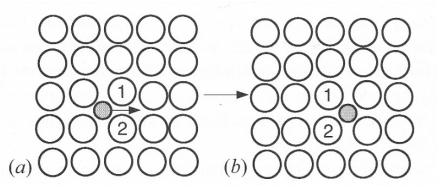
\includegraphics[width=0.8\textwidth]{Immagini/Inter.png}
    \caption
    {
        Example of diffusion of an interstitial atom inside a general simple lattice.
    }
    \label{fig:Inter}
\end{figure}
A practical example of such a phenomenon is the diffusion of Carbon inside Iron, or Hydrogen in a general material. Such movements are able to give the material particular properties or drive it to different equilibrium respect the one we imagine. Therefore, we want to focus on the study of atoms movements inside the material to create a good model for diffusion processes to then apply them into material modelling.

In order to do that we shall focus on the description of the flux of particles of $i$-th type, $\vb{J}_i$, inside the material, and we have seen that is related to the gradient of chemical potential. Still, we can see more in depth how they are related by defining a really important quantity called \textbf{mobility} as follows.
\dfn{Mobility}
{
    The mobility of atoms of type $i$, $M_i$, inside a material is constant of proportionality between the average particle velocity and the gradient of chemical potential
    \begin{equation}
        \left\langle \vb{v}_i \right\rangle = -M_i\grad \mu_i.
    \end{equation}
}
\noindent
Then, from this definition one can easily see how the flux and chemical potential are related since $\vb{J}_i$ is given by the density of that type of atoms $c_i$ multiplied by the average velocity, having
\begin{equation}
    \label{eq:fluxForm}
    \vb{J}_i = c_i \left\langle \vb{v}_i \right\rangle = -c_iM_i\grad \mu_i.
\end{equation}
Which is the relation we have seen in the previous part when talking about the $\mathcal{L}$ matrix. Still, we can work the expression a little more and see how in reality we can collect the flux at the gradient of concentration using the following result.
\thm{Fick's law}
{
    Inside a material, if the interstitial moving atoms are much less compared to the solvent atoms so that the system can be approximated to a dilute solution we can write the flux of atoms as
    \begin{equation}
        \vb{J}_i = -k_B TM_i\grad c_i = -D_i\grad c_i,
    \end{equation}
    where $D_i$ is also called \textbf{diffusion constant}.
}
\pf{Proof}
{
    Since the system can be thought of a dilute solution the Henry’s law can be used so that the chemical potential is
    \begin{equation}
        \mu_i = \mu_i^0 + k_BT\ln\left( \gamma_i^0X_i \right) = \mu_i^0 + k_BT\ln\left( \gamma_i^0\frac{N_i}{V}\frac{V}{N_T} \right) = \mu_i^0 + k_BT\left[ \ln\left( \frac{\gamma_i^0}{\left\langle c \right\rangle} \right) + \ln c_i\right].
    \end{equation}
    We can see how in this relation $\gamma_i^0/\left\langle c \right\rangle$ is a constant, so that by taking the gradient we have that a relation between $\mu_i$ and $c_i$ is obtained as
    \begin{equation}
        \grad \mu_i = \frac{k_BT}{c_i}\grad c_i.
    \end{equation}
    Then by substituting it inside \eqref{eq:fluxForm} the wanted relation is obtained, with also the important equality
    \begin{equation}
        D_i = k_BTM_i,
    \end{equation}
    which is also called \textbf{Nernst-Einstein relation}.
}

\subsection{Substitutional diffusion}

To be able to model the flux of a certain atomic spicy inside a material we need first to unravel the possible mechanisms that allow it to move in the first place. We have already discussed how one simple way in which an atom can move inside a solid is by moving in the interstitial positions inside the lattice. Nevertheless, this is valid only if the spicy we are looking at is small enough, and that is not the case for the majority of diffusion mechanisms inside a material. In particular, we now want to focus on the situation where no interstitial occupancy is present, and obviously also double occupancy of a site, and see how atoms of different types can move inside the lattice.

\begin{figure}[t]
    \centering
    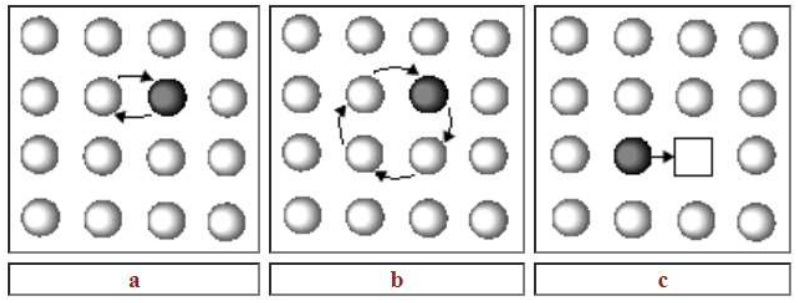
\includegraphics[width=0.8\textwidth]{Immagini/DiffMech.png}
    \caption
    {
        Representation of the three main possible diffusion mechanism, in order: direct exchange, cyclic exchange, and vacancy diffusion.
    }
    \label{fig:DiffMech}
\end{figure}
A lot of research was done in the past by several physicists working especially in the world of metallurgy, and to this day we know three main possible mechanisms that allow atoms to diffuse inside a lattice described in \figref{fig:DiffMech}. We can see how three mechanisms are described, where the atoms can exchange positions with one another, either with a \textbf{direct exchange} with one another or with a \textbf{cyclic exchange}, or by moving inside particular point defects called \textbf{vacancies}. The latter, in particular, result in being the most important mechanism of the three, able to describe a lot of physical phenomena. To understand this we need first to address the fact that before 1939 the only mechanism that was thought possible was the direct exchange so that a lot of constrains for the diffusion were present. For example, if we have an alloy formed by two atomic species the only possibility for the species to move respect to each other was to exchange places, so that for an atom of type A going in a direction one of type B was going in the opposite having
\begin{equation}
    \label{eq:FluxConstr}
    \vb{J}_A  + \vb{J}_B = 0.
\end{equation}
A really important scientist called Kirkendall showed how this identity was indeed not true, so that the fluxes of the two species inside an alloy could have different modules. 

Kirkendall took an ingot of Brass, an alloy composed by Cu and Zn, with a series of Molybdenum wires attached to it and then coat the structure with an outer layer of Copper. Then, he took the system to a temperature of \SI{785}{\celsius} and waited looking at how atoms will diffuse in the Copper. In fact, the main point was that at that temperature and concentration the Brass phase was stable, so that Zn atoms would travel in the outside part creating brass at lower concentration while also Cu atoms will travel inside to form Brass. Mo wires instead remained attached to the core during this process, since were not miscible, allowing to see if the core volume would change or not. If only the direct exchange mechanism was present then outside Zn flux would be the opposite of inward Cu one, meaning that the core should have remained the same in volume, but the experiment showed the situation in \figref{fig:KirkExper}.
\begin{figure}[t]
    \centering
    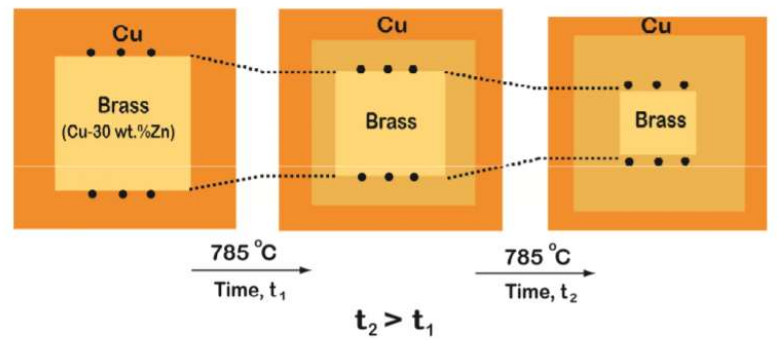
\includegraphics[width=0.8\textwidth]{Immagini/KirkExper.png}
    \caption
    {
        Results of the Kirkendall experiment showing how the Brass core becomes smaller due to different values of the fluxes for the two different atomic species.
    }
    \label{fig:KirkExper}
\end{figure}
In order to explain such a result the only possibility is to insert inside the computations the presence of a third spicy that is traveling inside the material, so that the relation \eqref{eq:FluxConstr} would have a larger degree of freedom. Thus, Kirkendall proposed that vacancies inside the material would actually work as the third species so that fluxes relation would be
\begin{equation}
    \vb{J}_A  + \vb{J}_B + \vb{J}_V = 0,
\end{equation}
allowing for what is now called the \textbf{Kirkendall effect} to happen. Therefore, the presence of vacancies inside a material is of a major importance in the description of the diffusion processes that are able to modify the concentration of atomic species inside it, as we will see.

\nt
{
    The diffusion of atoms inside a material is called substitutional diffusion since we can think of the phenomenon just described as atoms of different species respect the expected one are present inside the lattice, forming substitutional defects. Then those defects start to move inside the material varying the concentration of the several species, so in this optic we imagine defects as a type of atom so a particular substitutional defect. 
}

\subsection{Network constraint}

To study the evolution of atomic concentration inside a material we will need to make more formal the observation seen inside the previous discussion and see how they apply mathematically. In particular, we have seen how the main point reside on the fact that the fluxes are constrained due to continuity effect along with the nature of the direct exchange mechanism. This can be sad in a more formal way using the following result
\thm{Network constraint}
{
    Inside a material with $C$ different components we have that if we assume that the volume of the system is fixed and the site can be singly occupied or vacant, then the total number of entities must be locally conserved:
    \begin{equation}
        \label{eq:NetConstr}
        \sum_{i=1} ^{c+1} \dd N_i = 0.
    \end{equation}
    Where the $c+1$ count also the vacancies as a component.
}
\noindent
That result is of a major importance in the theoretical study of the diffusion processes since we can easily see how allows for the theoretical derivation of the constraint described in the Kirkendall effect. In fact, by recalling how the flux is defined one can easily write down the following
\begin{align}
    \label{eq:FluxResult}
    &\vb{J}_i = \pdv{N_i}{A}{t}\vb{n}, &\sum_{i=1}^{c+1}\vb{J}_i = 0,
\end{align}
where $\vb{n}$ is the normal vector to the surface $A$ over which we are evaluating the flux. Nevertheless, this is not the only use we have for such an expression, we can also see how the network constraint also implies that an arbitrary chemical potential con be use as a reference for the others. Basically, we can select a component $j$ and use \eqref{eq:NetConstr} to rewrite it's differential using the others, so that
\begin{equation}
    \dd N_j = -\sum_{i\neq j} \dd N_i,
\end{equation}
which can be substituted inside the form of the Gibb's free energy in order to have
\begin{equation}
    \label{eq:ConstrGibbs}
    G = \sum_{i=1}^{c+1}\mu_i \dd N_i = \sum_{i\neq j} \left( \mu_i - \mu_j \right)\dd N_i.
\end{equation}
This is telling us that we can choose one chemical potential of our choice, set it to zero, and scale the others based on that to work with basically one component less. Also, \eqref{eq:ConstrGibbs} shows how also the conjugates forces that relates to the $\dd N_i$ quantities, and so the fluxes, can be rescaled in terms of a component. Meaning that we can simply write the driving forces using the realtion
\begin{equation}
    \vb{F} = - \grad\left( \mu_i - \mu_j \right),
\end{equation}
simply the rescaled chemical potential gradient.

As a last remark, we can also see another interesting result. In particular, using the network constraint we can see how the $\mathcal{L}$ matrix posses more symmetry than what we expect having that the following is true.
\cor{$\mathcal{L}$ symmetry}
{
    In a system where the network constraint is valid we have that the following holds
    \begin{equation}
        \sum_{i=1}^{c+1} \mathcal{L}_{ij} = 0 = \sum_{i=1}^{c+1} \mathcal{L}_{ji}.
    \end{equation}
}
\pf{Proof}
{
    The proof is simple, we can simply use the definition of the matrix and the relation \eqref{eq:FluxResult} to obtain
    \begin{equation}
        \sum_{i=1}^{c+1}\vb{J}_i = \sum_{i=1}^{c+1} \sum_{j=1}^{c+1}\mathcal{L}_{ij}\vb{F}_j = \sum_{j=1}^{c+1} \left( \sum_{i=1}^{c+1}\mathcal{L}_{ij}\right)\vb{F}_j = 0, 
    \end{equation}
    since this must hold for an arbitrary value of the forces the element between parenthesis needs to be zero, and the Onsager's symmetry gives out the wanted result.
}

\subsection{Substitutional diffusivity}

Now, it's time to use what we have seen so far to create a mathematical simple model for diffusion. In particular, we are going to use a binary alloy and see how a model for diffusion can be obtained giving out a value for the diffusivity $D_i$ of a certain atomic species.
\thm{Diffusivity in a binary alloy}
{
    Inside a dilute binary alloy, with concentration gradient, the diffusivity of a component can be written as
    \begin{equation}
        \label{eq:BinaryDiff}
        D_i = k_BT\begin{cases}
            \left( \frac{\mathcal{L}_{11}}{c_1} - \frac{\mathcal{L}_{12}}{c_2} \right)\left( 1 + \pdv{\ln\gamma_1}{\ln c_1} + \pdv{\ln\left\langle V \right\rangle}{\ln c_1} \right), & i = 1\\
            \left( \frac{\mathcal{L}_{22}}{c_2} - \frac{\mathcal{L}_{21}}{c_1} \right)\left( 1 + \pdv{\ln\gamma_2}{\ln c_2} + \pdv{\ln\left\langle V \right\rangle}{\ln c_2} \right), & i = 2
        \end{cases}.
    \end{equation}
}
\pf{Proof}
{
    We know that in a binary alloy the total atomic species that we need to count are three, one of which are the vacancies. Therefore, we can use the result of the network constraint and set the chemical potential of the vacancies as the reference, having $\mu_V = 0$, and work on the other two. We can so use the Gibbs-Duhem equation in this situation and divide the relation for the volume $V$ to have
    \begin{align}
        &c_1\dd \mu_1 + c_2 \dd\mu_2 = 0, &\dd \mu_1 = -\frac{c_2}{c_1}\dd \mu_2,
    \end{align}
    where $\dd \mu_V = 0$ since $\mu_V$ was set to the constant value of zero. Then, we can use the constitutive relations $\vb{J} = \mathcal{L}\vb{F}$ to write down a form for the fluxes inside the material in a general way as
    \begin{align}
        &\vb{J}_1 = -\mathcal{L}_{11} \grad \mu_1 - \mathcal{L}_{12} \grad \mu_2,
        &\vb{J}_2 = -\mathcal{L}_{21} \grad \mu_1 - \mathcal{L}_{22} \grad \mu_2.
    \end{align}
    We can then take the flux for the first atomic type and substitute the gradient of $\mu_2$ in order to obtain
    \begin{equation}
        \label{eq:DiffAllPf}
        \vb{J}_1 = -\left( \mathcal{L}_{11} - \frac{c_1}{c_2}\mathcal{L}_{12} \right)\grad \mu_1.
    \end{equation}
    Then, the Henry's law form for the chemical potential can be used so that we can explicitly write down the gradient as
    \begin{align}
        &\mu_1 = \mu_1^0 + k_B T \ln\left( \gamma_1X_1 \right) = \mu_1^0 + k_B T \ln\left( \gamma_1\frac{N_1}{V}\frac{V}{N_T} \right) = \mu_1^0 + k_BT\left( \ln\gamma_1 + \ln\left\langle V \right\rangle + \ln c_1 \right).
    \end{align}
    We will assume that $\gamma_1$ and $\left\langle V \right\rangle$ will depend on position by the value of $c_1$ so that we can evaluate the gradient simply as
    \begin{equation}
        \grad \mu_1 = \frac{k_BT}{c_1}\left( 1 + \pdv{\ln\gamma_1}{\ln c_1} + \pdv{\ln\left\langle V \right\rangle}{\ln c_1} \right).
    \end{equation}
    By substituting inside \eqref{eq:DiffAllPf} and confronting with Fick's law $\vb{J}_i = -D_i \grad c_i$ we are able to obtain the wanted result. The procedure is analogous for the other component.
}
\noindent
In this way we are able to describe the evolution of the species by using Fick's law, seeing how the fluxes goes in the directions opposites to the gradient of concentration. Meaning that atoms goes in the direction where they are less and the two of them can have different velocities, since the difference between the two is compensated by the vacancy flux. Also, often \eqref{eq:BinaryDiff} is simplified since the diagonal components of $\mathcal{L}$ are generally larger than the off-diagonal once and $\left\langle V \right\rangle$ is usually nearly constant meaning that for the case of the first component one can write 
\begin{equation}
    D_1 \approx \frac{k_BT\mathcal{L}_{11}}{c_1}\left( 1 + \pdv{\ln\gamma_1}{\ln c_1} \right).
\end{equation}
Where the term with $\gamma_1$ represent the level of non ideality of the solution. Also, another specific case is when the second type of atoms $1^*$ is taken as an isotope of the other one, so that the solution is surely ideal and the diffusivity becomes
\begin{equation}
    D_{1}^* = k_BT\left( \frac{\mathcal{L}_{11}}{c_1} - \frac{\mathcal{L}_{11^*}}{c_{1^*}} \right),
\end{equation}
which is also called \textbf{self diffusivity}. Usually also the off-diagonal term $\mathcal{L}_{11^*}$  it's pretty small having that at last the approximation of $D_1$ can be stated in terms of the self diffusivity as 
\begin{equation}
    D_1 \approx D_{1}^*\left( 1 + \pdv{\ln\gamma_1}{\ln c_1} \right).
\end{equation}
Meaning that the diffusion properties of a species can be seen as the one for its diffusion in itself plus the non ideality of the solution in which is present.

All of these equations have implicitly used a system of reference attached to the crystal lattice, the C-frame, since we have always considered the movements of the atoms relatives to the atomic positions themselves. It is also possible, and useful, to restate the theory using the system of reference of the laboratory where the volume of the sample is fixed in space called the V-frame, and is defined by assuming the ends of the sample at rest, not moving, and so fixed volume. In this frame of reference it's possible to see some results, like the relative velocity given by
\begin{equation}
    \vb{v}_C^V = \left( D_1 - D_2 \right)\overline{V}_1 \grad c_1.
\end{equation}
Another important property that can be seen of the movements inside the V-frame is that the two components of a binary alloy present the same diffusivity, called \textbf{interdiffusivity} defined as
\begin{equation}
    \tilde{D} = c_1\overline{V}_1 D_2 + c_2\overline{V}_2D_1.
\end{equation}
So, the diffusivity in this situation is the same for both the species, but the fluxes can still be different due to different concentration gradients.

\subsection{Vacancies in equilibrium}

We have seen how vacancies are probably the most important point defect that we need to focus on in order to describe the diffusion mechanism inside a material. For this reason is interesting to see how effectively they appear and how many of them are present. The latter, in particular, can be addressed in a simple way by using equilibrium thermodynamic in order to see the molar fraction of vacancies that minimize the free energy of a system. Giving rise the result reported next.
\thm{Vacancy presence}
{
    In a material composed by $N_A$ atoms and $N_V$ vacancies, if we have $N_V \ll N_A$, we have that at equilibrium the molar fraction of vacancies is
    \begin{equation}
        X_V = \exp\left( -\frac{G_V^f}{k_BT} \right) = \exp\left( \frac{S_V^f}{k_B} \right)\exp\left( -\frac{H_V^f}{k_BT} \right),
    \end{equation} 
    where $G_V^f$ is the variation of free energy needed in order to form the vacancy in the crystal.
}
\pf{Proof}
{
    We can write down the free energy of the system by adding to the free energy of the single component the increase of entropy given by using Bragg-Williams-Gorsky configurational entropy once again, and having
    \begin{equation}
        G = N_A\mu_A^0 + N_V G_V^f + k_BT\left[ N_A\ln\left( \frac{N_A}{N_A + N_V} \right) + N_V\ln\left( \frac{N_V}{N_A + N_V} \right) \right].
    \end{equation}
    From this we use the fact that $N_V \ll N_A$ and evaluate the chemical potentials of the two components having
    \begin{align}
        &\mu_A = \pdv{G}{N_A} \approx \mu_A^0, &\mu_V = \pdv{G}{N_V} \approx G_V^f + k_BT\ln X_V.
    \end{align}
    At equilibrium, we need $\partial G/\partial N_V = 0$ meaning that we can obtain the wanted relation by simply setting $\mu_V = 0$ and inverting it.
}
\noindent
It's interesting because the value of $X_V$ can be experimentally measured by differential difrattometry at different temperatures, where the variation of the volume can be obtained and then the one that comes from thermal expansion can be omitted by evaluating the lattice constant using diffraction. Still, $X_V$ can be computed and so by doing a logarithmic fit one can obtain the value of $H_V^f$ which can be useful for some other investigations, also the general values are around \SI{0.65}{\electronvolt}.

Still, this result is leaving behind some questions. In fact, it seems strange that the vacancies can have a constant value at equilibrium if still a constant flux is present inside the material which would lead to elimination of them in time. It's not easy to imagine how vacancies traveling inside a material at a constant speed would at the end arrive at the surface where they will simply become a surface defects eliminating one vacancy. For this reason having a constant value of $X_V$ is implying that center of creation of vacancies needs to be present inside the material, and can be seen how this is actually true the source being \textbf{dislocations}.

\subsection{Dislocations in crystals}

Dislocations are line defects inside materials that are created due to external pressure pushing the sides of the sample in an uneven way moving the lines of atoms in different positions. The best way to understand the latter description is by using the \textbf{Burger's circuit} construction for the definition of such defects in a structure. Basically the idea is to draw a cyclic rectangular line on the surface of the material, and in case no defects are present the cycle will close, otherwise the vector missing completing the line is called \textbf{burger vector} and define the entity of the dislocation alongside with the direction. An example of that is shown in \figref{fig:Burg} where the two major types of dislocations are depicted by the drawing of the Burger circuit, still in reality the situation is more complex than that having dislocations that are a mix of those two but it's good to have an image of how they look like.
\begin{figure}[t]
    \centering
    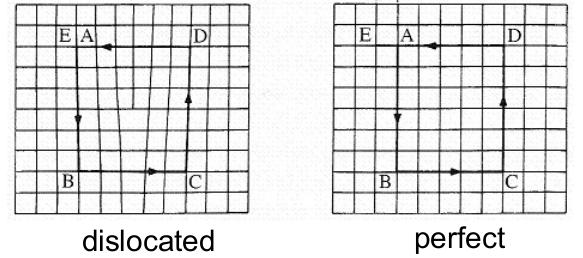
\includegraphics[width=0.6\textwidth]{Immagini/Burg1.png}
    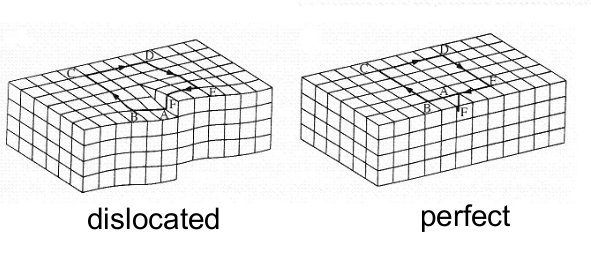
\includegraphics[width=0.6\textwidth]{Immagini/Burg2.png}
    \caption
    {
        Construction of Burger's vectors in two different types of dislocations: edge dislocations on top, and screw one on the bottom. 
    }
    \label{fig:Burg}
\end{figure}

Nevertheless, we are interested in the description of how such line dislocations can be thought as creators of vacancies, and to understand that we need to talk about how dislocations can move inside a crystal. In fact, dislocations are able to change positions inside a lattice by using two main movements: \textbf{glide}, and \textbf{climb}. The former is a simple situation where a shear pressure is applied to the lattice and in the direction of the Burger's vector so that the dislocation start gliding on the side of the material, as its possible to see in \figref{fig:DisMov}.
\begin{figure}[t]
    \centering
    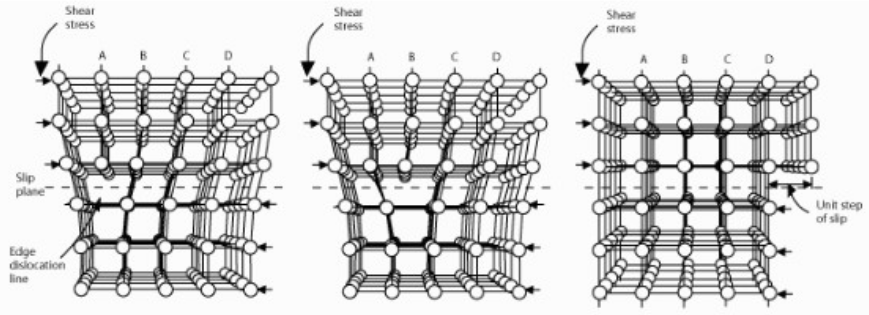
\includegraphics[width=0.7\textwidth]{Immagini/DisMov1.png}
    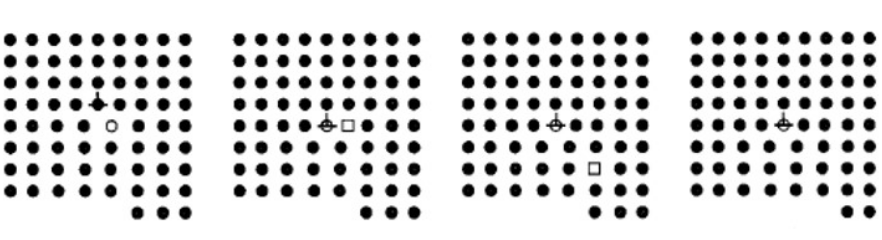
\includegraphics[width=0.7\textwidth]{Immagini/DisMov2.png}
    \caption
    {
        Graphical representation of the two types of dislocations movements: glide movement on top, climb movement on the bottom. In particular, the climb movement bring the dislocation down in this case.
    }
    \label{fig:DisMov}
\end{figure}
Still, such movements isn't able to produce vacancies, it's more important for the possibility of eliminating defects bringing dislocations to the edge of the material recreating symmetry in the bulk. The real movement that we are interested in is so the climb one. We can see, always from \figref{fig:DisMov}, how the climb movement instead of moving the dislocation to the side is able to bring it up or down in extension. In particular, the way in which this happens requires for atoms around the dislocation to move in order to position themselves into the dislocations, to increase the extent, or out of it, decreasing it. In both cases for the atoms to move in other positions we need that vacancies are involved, in fact if atoms would swap places with another one nothing would happen. Therefore, if the dislocation increase in extent an atom from the symmetric lattice need to enter the dislocation line leaving behind a vacancy, \textbf{generating them}, instead if we have a decrease an atom need to go into a vacancy, \textbf{destroing them}. Basically, through the climbing mechanism the \textbf{dislocations can be seen as both sources and sink of vacancies}, giving rise to a non-conservative motion that involves atomic diffusion.

We have so seen how effectively vacancies can be created inside a material understanding how effectively is possible that a constant fraction of them is present at equilibrium. Still, dislocations posses also other properties that influences the diffusion inside the material. In particular, is possible to understand that due to the variation of lattice near the defect also a pressure gradient is created that tries to separate the part under the dislocation and unite the one above it. That pressure gradient, called \textbf{Cottrell atmosphere} at equilibrium, is felt by the atoms in the surroundings creating variation in the flux that can be inserted using the following expression
\begin{equation}
    \vb{J}_i = -D_i\left( \grad c_i + \frac{c_i \Delta \overline{V}_i}{k_BT}\grad P \right),
\end{equation}
where $\Delta \overline{V}_i$ is the local variation of the volume occupied by the $i$-th spicy due to the dislocation. This can be also described by the substitution of the chemical potential as the designed one to generate the flux to an \textbf{elastochemical} one that is defined as
\begin{equation}
    \Phi_i = \mu_i + \Delta \overline{V}_i P,
\end{equation}
and use that in the computations. This idea of redefining the potential to include effects inside the diffusion mechanism is a really valid one that we are going to use also further in the course. For this reason we will anticipate the form for the diffusion potential inside an ionic crystal, where the electrostatic forces between atoms needs to be taken into account for diffusion giving rise to
\begin{equation}
    \Phi_i = \mu_i + q_i\phi.
\end{equation}
Where $\phi$ is the electrical potential present in the crystal and the total potential is so-called \textbf{electrochemical diffusion potential}.